\section{Mixtures of Experts Models}
\label{CH:ExpertModels}

Mixture of experts models cover a wide range of mixture models where multiple expert candidates compete for best performance. Consider yourself a forecaster and you have a certain number of experts or candidates for advice around you and you want to combine or mix their advice into one prediction. The mixture components can be modelled by covariates or functions of the individual candidate's performance.
Having its origin in the machine learning literature, they do appear in many guises \citep{gormley2018mixtures}. The main goal is to predict a unknown sequence $y_1, y_2, ... $ of independent and identically distributed outcome variables. Subject to a loss function, a natural forecasting strategy would be to combine the experts' predictions $\hat y_t^{k}$, $t = 1, 2, ...$ in a weighted average to get the aggregate forecaster's predictions $\hat y_1, \hat y_2, ...$, where $k$ is referring to one of the experts, while keeping the \textit{cumulative regret} (or simply \textit{regret}) with respect to each expert small. The performance of each expert is evaluated subject to a loss function $L: \R^2 \to \R_{>0}$, $(\hat y_t, y_t) \mapsto L(\hat y_t, y_t)$ which enables the definition of the regret as \citep{CesaBianchi2006PredictionLearningGames}
\begin{equation}
    R_n^k = \sum_{t=1}^{n} \left(L(\hat y_t, y_t)-L(\hat y_t^{k},y_t)\right) = \hat L_n - L_{k,n} \label{EQ:Regret}
\end{equation}
where $\hat L_n$ is the forecaster's cumulative loss and $L_{k,n}$ is the cumulative loss of expert $k$. Accodingly, the instant regret to expert $k$ can be defined by $r_{k,t} = L(\hat y_t, y_t)-L(\hat y_t^{k},y_t)$. One can interpret this quantity as the regret the forecaster feels for not having listened to the advice of expert $k$ in the prediction of $y_t$. The main motivation for the employment of multiple experts over a single candidate is the expectation that an ensemble outperforms a single expert (\textit{The wisdom of crowds}). In this sense, the regret should vanish for an increasing number $n$ of observations. That is
\begin{equation}
    \frac{1}{n}\left(\hat L_n - \min_{k} L_{k,n}\right) \to 0 
\end{equation}
for $n\to\infty$. The performance and the ensurance of this goal can only be evaluated in hindsight but regret bounds do exist for different algorithms.

Hence, assume we have finite number $K \in \N$ of possible experts or components and a weighting $\bw_t = \left(w_t^1, ..., w_t^K\right) \in \left[0,1\right]^{K}$ ($t=1,2,...$) at time $t$ of those experts such that $\sum_{k=1}^{K} w_t^k = 1$ for all $t$. Each expert $k$ ($k= 1, ... , K)$ produces a forecast, which in its most general form can be described by a density $f_k(\cdot \,|\, \theta_k)$ depending on a parameter $\theta_k(\bx_t)$ which can be based on a set of covariates $\bx_t$ \citep{gormley2018mixtures}. The goal is to sequentially find a good weighting $\bw_t$ of the experts to combine their predictions. On the basis of the experts' predictions, a final prediction is computed as

\begin{equation}
    p(y_t \,|\, \bx_t) = \sum_{k=1}^{K} w_k f_k(y_t \,|\, \theta_k(\bx_t))
\end{equation}

This model, by allowing $\bw_t$ and $\theta_k(\bx_t)$ to vary in different ways, allows for a wide range of applications, one of which we want to highlight in the following section.

One common way to model $\bw_t$ and $\theta_k(x_t)$ is to choose a point forecast $\hat y_t^{k}$ instead of a density $f_k ( y_t \,|\, \theta_k(x_t))$. The forecaster chooses a weighting $\bw_t$ of the experts and combines their individual point forecasts $\hat y_t^{k}$ by
\begin{equation}
    \hat y_t = \sum_{k=1}^{K} \bw_t^{k} \hat y_t^{k}
\end{equation}
and - by observing the true value $y_t$ - suffers a non-negative loss $L(\hat y_t, y_t)$. Now the performance of each expert can be judged based on the loss function $L$ or equivalently on each expert's regret $R_n^k$ from \refp{EQ:Regret}.


\subsection{Loss Induced Weighting of Experts}
\label{CH:ExpertModels:Loss}

It seems intuitive to update the weighting of the experts based on their performance, such that an expert with a high regret receives a higher weight because it would have been advisable to 'listen' to him and an expert with a comparably lower regret receives a lower weight. This can be achieved by different approaches \citep{CesaBianchi2006PredictionLearningGames}
\begin{eqnarray}
    \text{Linear:} & w_t^k = & \frac{R_t^k}{\sum_{i=1}^K R_t^{i}} \\
    \text{Polynomial:} & w_t^k = & \frac{2(R_t^k)_{+}^{p-1}}{\left(\sum_{i=1}^K (R_t^{i})^p\right)^{(p-2)/p}} \\
    \text{Exponential:} & w_t^k = & \frac{\exp{\eta R_t^k}}{\sum_{i=1}^{K} \exp{\eta R_t^i}}
\end{eqnarray}
to differently weight the regret where the fractions are needed to normalize the weights to ensure $\sum_{k=1}^{K} w_t^k = 1$. $( \, \cdot \,)_{+}$ is referring to the positive part, so $(x)_{+} = \text{max}\left\{0, x\right\}$. The exponential update introduces a learning rate $\eta > 0$ which bears a drawback of the exponential weighting because of the introduction of a hyperparameter that may be subject to optimization. Nevertheless, we will focus on this approach because of its nice properties and the similarity to the plasticity weighting which we will introduce in section \ref{CH:ExpertModels:Plasticity}. One major advantage of the exponentially weighted approach is the fact that it can be equivalently formulated as an incremental update of the weights by inserting \refp{EQ:Regret}
\begin{eqnarray}
    w_t^k & = & \frac{\exp{\eta R_t^k}}{\sum_{i=1}^{K} \exp{\eta R_t^i}} \\
    & = & \frac{\exp{\eta \sum_{\tau=1}^{t} \left(L(\hat y_\tau, y_\tau)-L(\hat y_\tau^{k},y_\tau)\right)}}{\sum_{i=1}^{K} \exp{\eta \sum_{\tau=1}^{t} \left(L(\hat y_\tau, y_\tau)-L(\hat y_\tau^{i},y_\tau)\right)}} \\
    & = & \frac{w_{t-1}^k\exp{\eta \left(L(\hat y_t, y_t)-L(\hat y_t^{k},y_t)\right)}}{\sum_{i=1}^{K} w_{t-1}^i\exp{\eta \left(L(\hat y_t, y_t)-L(\hat y_t^{i},y_t)\right)}} \\
    & = & \frac{w_{t-1}^k\exp{-\eta L(\hat y_t^{k},y_t)}}{\sum_{i=1}^{K} w_{t-1}^i\exp{-\eta L(\hat y_t^{i},y_t)}} \label{EQ:LossUpdate} 
\end{eqnarray}
This update of weights only requires the last performance of the experts as opposed to the linear or polynomial update that depend on the regret and therefore on past predictions $\hat y_s^k$, for $s < t-1$ and $k = 1, ..., K$. Different choices of $\eta$ can lead to different performance results and one can circumvent its optimization by knowledge of the forecasting horizon which can help to choose $\eta$ in advance.


% Elaborate more on the regret.
One objective of the forecaster is to choose the learning rate of any algorithm for $w_t$ such that the regret is low. \cite{CesaBianchi2006PredictionLearningGames} prove different performance bounds for the weight updates mentioned above. The exponential update for a convex loss function $L: \R^2 \to [0,1]$ is proven to be
\begin{equation}
    \hat L_n - \min_{k=1,...,K} L_{k,T} \leq \frac{\log{K}}{\eta} + \frac{T\eta}{8} \label{EQ:OptimalLearningRate}
\end{equation}
for any $T > 0$ referring to the number of observations and any $\eta > 0$. Minimizing this upper bound with respect to $\eta$ one can choose $\eta = \sqrt{8\log{K}/T}$ which results in the minimal upper bound of $\sqrt{(T/2)\log{K}}$. This procedure, however, requires prior knowledge of the forecasting horizon $T$. If this is not known in advance, \cite{CesaBianchi2006PredictionLearningGames} further propose a time dependent learning rate $\eta_t$ that has a regret bound that holds uniformly over time. By choosing
\begin{equation}
    \eta_t = \sqrt{8\ln{K}/t}
\end{equation}
which comes back to an argument of resetting the optimal learning rate in \refp{EQ:OptimalLearningRate} after every prediction and considering only 1-step ahead prediction horizons, the regret bound becomes ....... % TODO March 16, 2020 : insert regret bound


\subsection{Pre-Prediction Update of Weights}

One of the main drawbacks of the loss induced expert weighting introduced in section \ref{CH:ExpertModels:Loss} is the fact that the weighting of the experts can be adjusted \textit{after} the loss has been suffered, i.e. after the prediction. To our knowledge, no research in this specific setting has been undertaken so far to update the weights of a set of Echo State Networks \textit{prior} to the prediction step. Coming up with measures to judge an expert's expected performance seems difficult but different sources lead to main part of this thesis which tackles this problem.

\subsubsection{Gaussian Mixture Autoregressive Model}
\label{CH:ExpertModels:GMM}

\cite{Kalliovirta2015GMUnivariateSeries} present a Gaussian Mixture Autoregressive Model (GMAR) where they use a particular choice of the mixing weights for a set of $K \in \N$ experts, each of them being an auxiliary, stationary AR(p) process. The stationary solution of such an AR(p) process specifies a mean value and an autocovariance structure on the time series. The mixing of those processes (experts) is based on the likelihood that the last $p$ observations of the target time series have been generated by any of those processes. Set ${\bf y}_{t-1} = \left(y_{t-1},...,y_{†-p}\right) \in \R^{p}$. They use the multivariate normal distribution $\mathcal{N}(\bmu^{k}, \Sigma^{k})$, $\mu^{k} \in \R^{p}$ and $\Sigma^{k} \in \R^{p\times{}p}$ for $k = 1, ..., K$, with density
\begin{equation}
    f^{k}(\by_{t-1}) = \frac{1}{\sqrt{(2\pi)^k \vert \Sigma^{k} \vert}} \text{exp}\left(-\frac{1}{2}\left(\by_{t-1}-\bmu^{k}\right)'(\Sigma^{k})^{-1}\left(\by_{t-1}-\bmu^{k}\right)\right)
\end{equation}
Subject to a mean weight $\balpha = \left(\alpha_1, ..., \alpha_K\right) \in \R^{k}$, they define the mixing weights $\alpha_{k,t}$ as
\begin{equation}
    \alpha_{k,t} = \frac{\alpha_k f^{k}(\by_{t-1})}{\sum_{i=1}^{K} \alpha_i f^{i}(\by_{t-1})}
\end{equation}

This method of weight update is - as within the expert setting - performed before the predition of the next value as one has uses the observations up to $y_{t-1}$ in order to predict $y_t$ which makes the process $\by_t$ Markovian.

\subsubsection{Echo State Incremental Gaussian Mixture Network}
\label{CH:ExpertModels:ESIGMN}

Another, very rich, line of research is \citep{Engel2010IncrementalGaussianMixtures, Heinen2011IGMN, Heinen2011ACA}. In one of their publications, \cite{ESIGM2011} propose a novel algorithm for incremental temporal pattern processing called the Echo State Incremental Gaussian Mixture Network (ESIGMN). It combines Echo State Networks with the Incremental Gaussian Mixture Network (IGMN) from \cite{Heinen2011IGMN}. 

The Incremental Gaussian Mixture Network is composed of multiple sets of virtual neurons (referred to as cortical regions), all of which have size $M \in \N$ and an association region. Figure \refp{FIG:IGMN} from their paper visualizes the model. 

\begin{figure}
    \begin{center}
    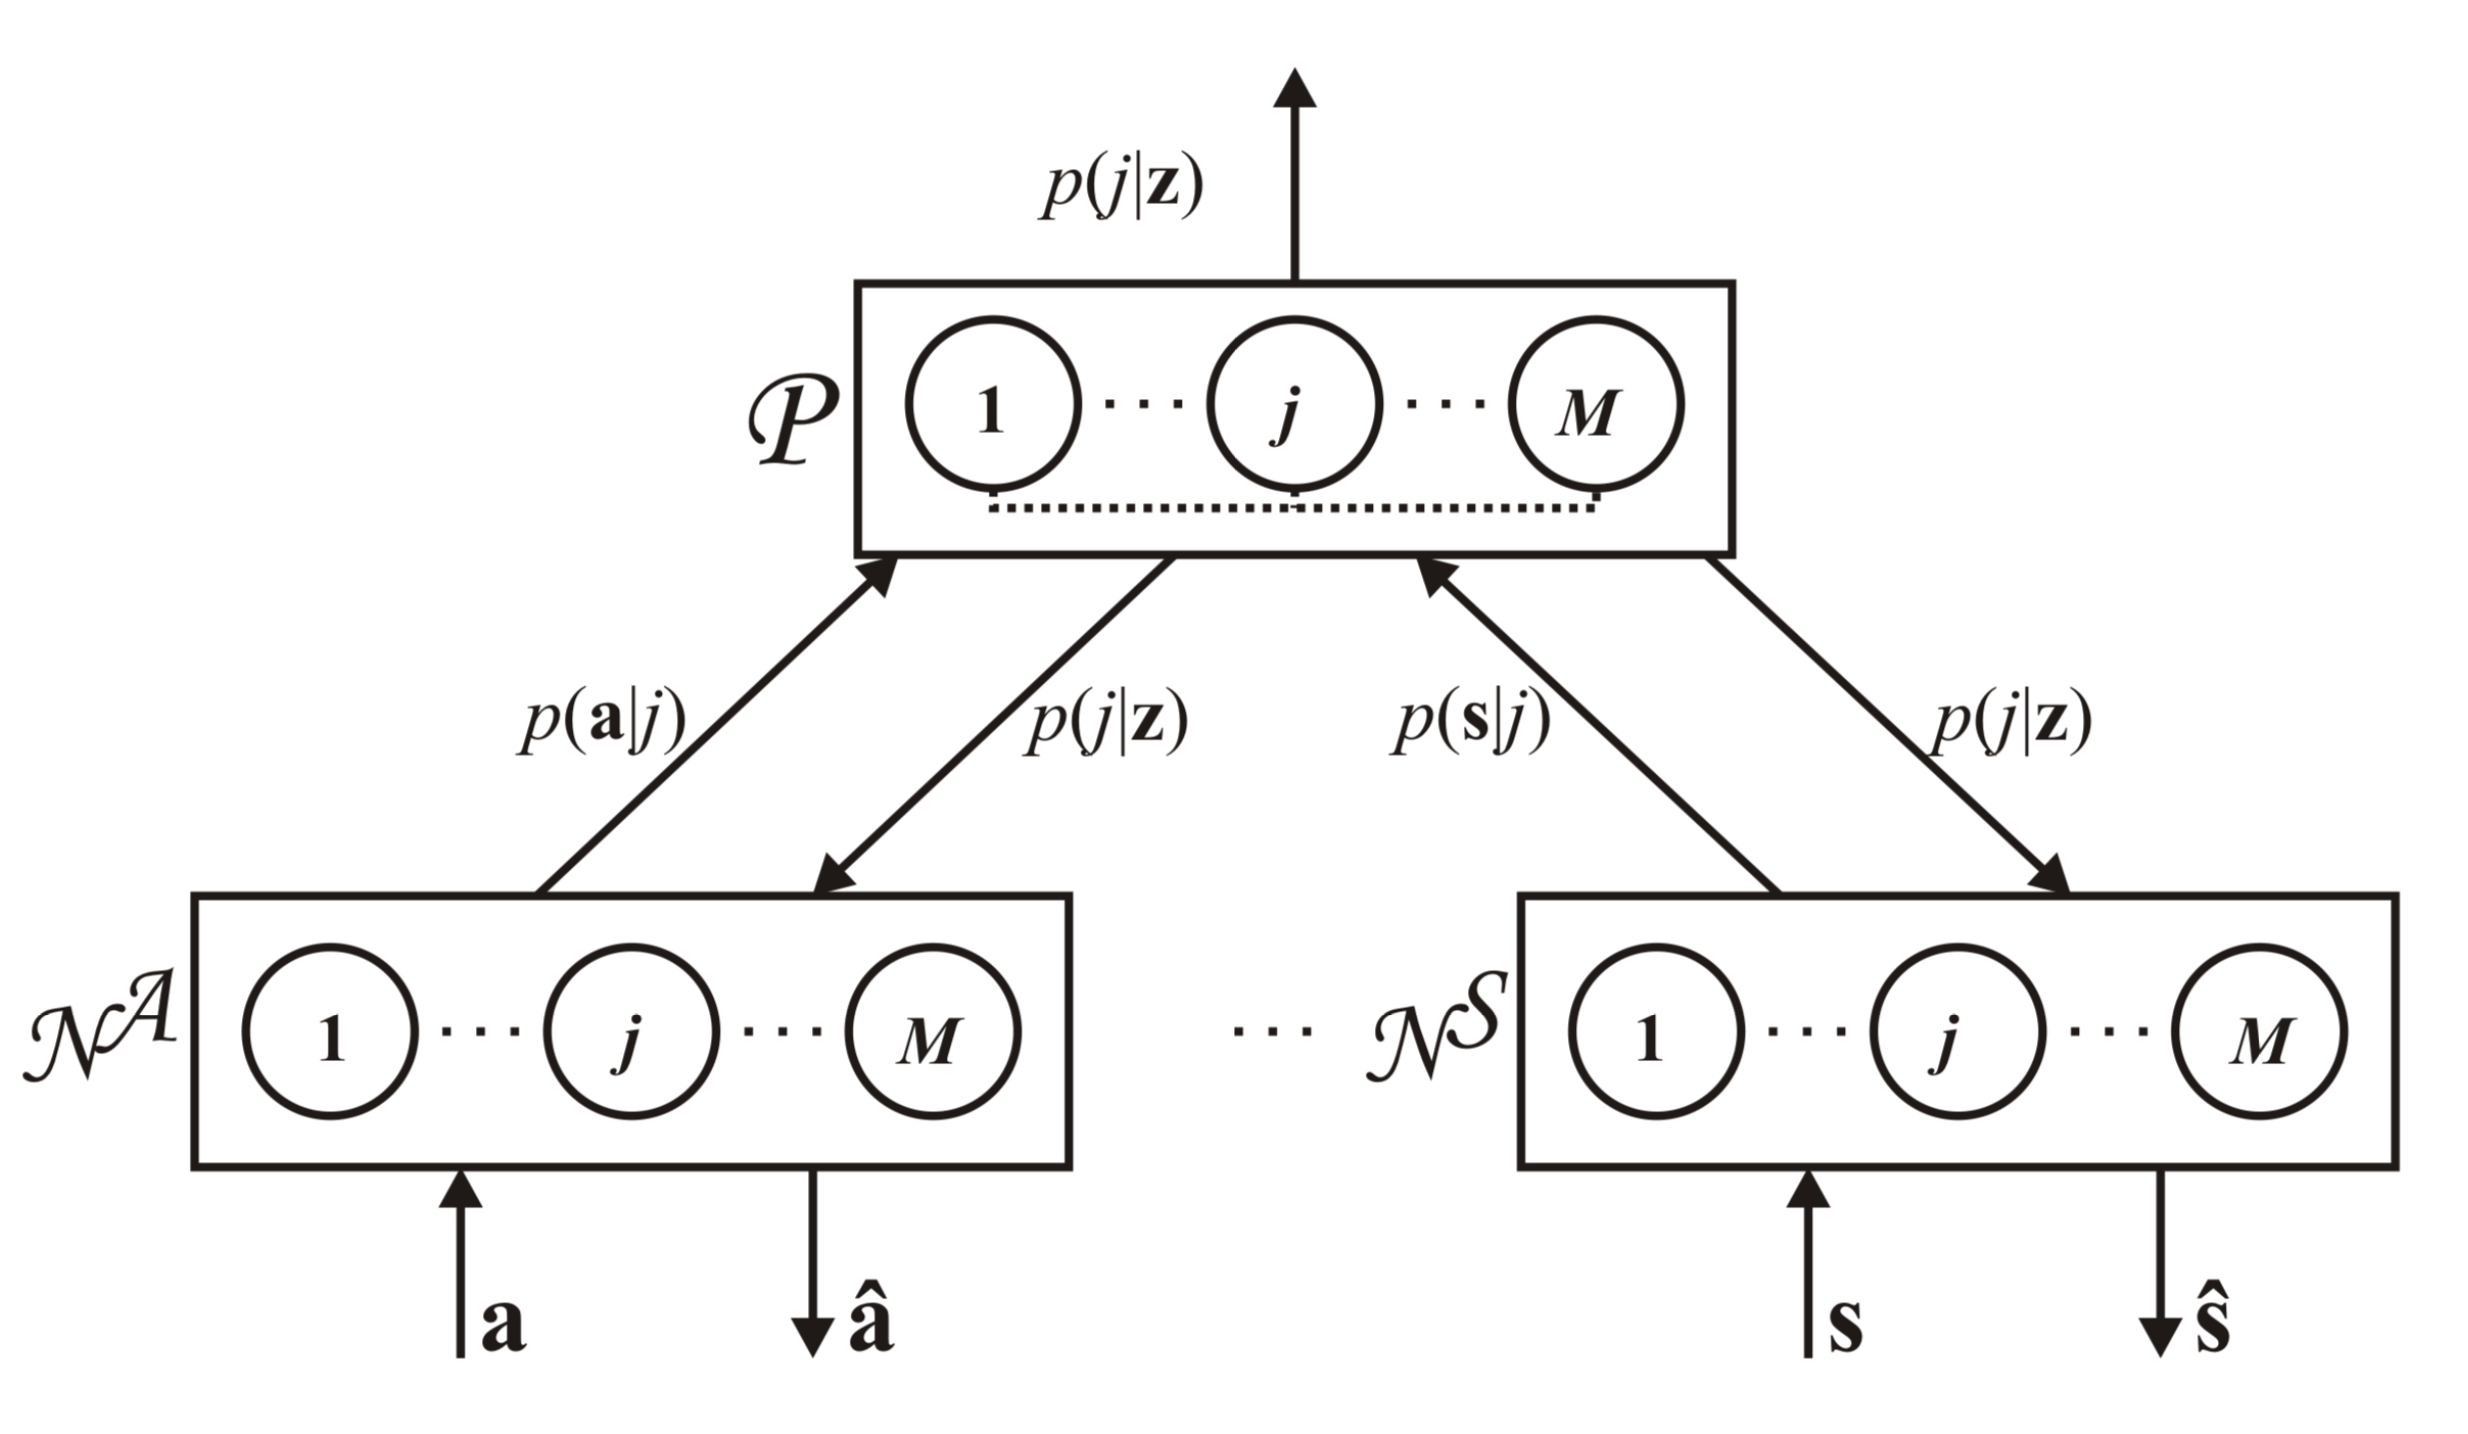
\includegraphics[width=0.7\textwidth]{Pictures/IGMN_Structure.png}
    \end{center}
    \label{FIG:IGMN}
    \caption{Basic architecture of the Incremental Gaussian Mixture Network from \cite{Heinen2011IGMN}. $\mathcal{N}^{\mathcal{A}}$ to $\mathcal{N}^{\mathcal{S}}$ refer to the coritcal regions and $\mathcal{P}$ is the association region. The cortical regions are only connected via the association region. New inputs are denoted by ${\bf a}$-${\bf s}$.}
\end{figure}

The IGMN is a gaussian mixture model with an agressive learning process, meaning the training data only has to be presented once. Based on $K \in \N$ distribution components (these are the \textit{cortical regions}) the network can adapt to the information from a new data point. One can think of the cortical regions as individual neural networks. Presented with a new input $u$\footnote{The notation has been adjusted to match our setting so far.}, a running mean $\mu_k$ and running covariance $\Sigma_k$ of network activations for each network are maintained\footnote{For details on the exact update of $\mu_k$ and $\Sigma_k$, the reader is referred to their paper.}. Based on these, the likelihood of each component $k$ is can be calculated:

\begin{equation}
    p \left(u \, | \, k\right)= \frac{1}{(2\pi)^{M/2}\sqrt{\abs{\Sigma_k}}} \exp{-\frac{1}{2}(u - \mu_k)'\Sigma_k^{-1}(u-\mu_k)}
\end{equation}

where $M$ is the size of component $k$. Given a prior distribution $p(k)$ which is initialized as $p(k) = \frac{1}{K}$ ($k = 1, ..., M$) posterior probabilites can be calculated for each component

\begin{equation}
    p(k \, | \, u) = \frac{p \left(x \, | \, k\right) p(j)}{\sum_{k=1}^{K} p \left(x \, | \, k\right) p(k)} \label{EQ:ESIGMN:posterior}
\end{equation}

The prior distribution $p(k)$ is also updated based on \refp{EQ:ESIGMN:posterior}. The recostruction of a target signal by the network is then produced as a weighted average of the individual regions' predictions 

\begin{equation}
    \hat y = \sum_{k=1}^{K} p(k \, | \, u) \hat y_m
\end{equation}

Where $\hat y_m$ is the prediction of the $m$-th component based on a Gaussian Process Regression. We will refrain from going into more detail, the interested reader is referred to their paper.

The further enhancement of \cite{ESIGM2011} to this idea is the preprocessing of the input $u$ by a single Echo State Network and the application of the Incremental Gaussian Mixture Network after the input has been transformed into a higher-dimensional representation.


\subsubsection{Plasticity based Weighting}
\label{CH:ExpertModels:Plasticity}

Both of the approaches outlined above are working with a likelihood based methodology to weight the predictions of a set of models (experts). As opposed to the loss induced weighting of experts, they choose the likelihood as a measure that is not related to the actual prediction error or loss, that the components suffer indivually. Accordingly, their model designs favour such an approach. 

To transfer this idea of a likelihood based weighting, the combination of \cite{Schrauwen2008}, \cite{Kalliovirta2015GMUnivariateSeries} and \cite{ESIGM2011} inspired a weighting of experts of echo state networks that is updated prior to the prediction step and is not necessarily dependent on a loss function $L$.

Given $K \in \N$ experts, each being an Echo State Network, we define $\bsigma := \left(\sigma_1, ..., \sigma_K\right)$, $\bmu := \left(\mu_1, ..., \mu_K\right) \in \R^{K}$. Assume we have tuned each of the networks by the approach of \cite{Schrauwen2008} with a target normal distribution $\mathcal{N}(\mu_k, \sigma_k^2)$ for $k = 1, ..., K$. Associated to these experts is a weight vector $\bw_t = \left(w_t^{1}, w_t^{2}, ..., w_t^K\right)$ where the index $t$ corresponds to a point in time.
After the network has been presented a new input and has been update to reflect the state $\bx_t$, the update of $\bw_t$ is based on the likelihood. Accordingly, weights are updated in the following way

\begin{eqnarray}
    \tilde w_{t}^{k} & = & p(x_t^k \, | \, \mu_k, \sigma_k^2) \nonumber \\ 
    & = & w_{t-1}^{k} \frac{1}{\sqrt{2\pi\sigma_k^2}} \exp{- \frac{\left(x^{k}_{t} - \mu_k\right)'\left(x^{k}_{t} - \mu_k\right)}{2\sigma_k^2}} \label{EQ:Likelihood}\\
    & & \text{for } k = 1,..., K \nonumber \\
    \bw_t & = & \frac{\tilde \bw_t}{\sum_{k=1}^{K}\tilde w_t^k}
\end{eqnarray}

This makes intuitive sense because the $k$-th Echo State Neworks has been tuned to follow a normal distribution with mean $\mu_k$ and variance $\sigma_k^2$ and, thereby, to achieve an information-maximization. Ranking the networks by their states' likelihood is equivalent to using the Kullback-Leibler divergence that has originally been used to move the network towards the targeted distribution.
As argued in section \ref{CH:ESN:Tuning}, $\mu_k$ can be set to $0$ and $p(\cdot \, | \, \mu, \sigma_k^2)$ refers to the density of a normal distribution with the given parameters\footnote{As will further be elaborated on in section \ref{CH:Application}, numerical accuracy in the calculation of \refp{EQ:Likelihood} can become critical, when the size $N$ of neurons in each expert gets large.}.
Let $N \in \N$ be the number of total neurons aggregated over all experts and $n = \frac{N}{K}$ be the size of one expert, define $\win^k$, $W^k$, $\wout^k$ and $\bb^k$ like in section \ref{CH:ESN:Architecture} and initialize $\bx_0^k = {\bf 0} \in \R^{n}$. We can outline the algorithm for the plasticity weighted experts of Echo State Networks

\begin{eqnarray}
    \bx_{t}^k & = & f\left(W^k\bx_{t-1}^k + \win^k u_t +  \bb^k\right) \\
    \tilde w_{t}^{k} & = & w_{t-1}^{k} \frac{1}{\sqrt{2\pi\sigma_k^2}} \exp{-\frac{\left(\bx^{k}_{t} - \mu_k\right)'\left(\bx^{k}_{t} - \mu_k\right)}{2\sigma_k^2}} \label{EQ:PlasticityWeightUpdate}\\
    & & \text{for } k = 1, ..., K \nonumber \\
    \bw_t & = & \frac{\tilde \bw_t}{\sum_{k=1}^{K}\tilde w_t^k} \\
    \hat y_t & = & \sum_{k=1}^K w_t^k \bx_{t}^k\wout^k \label{EQ:PlasticityPrediction}
\end{eqnarray}

For the ease of notation, the addition of an intercept or the input $u_t$ into \refp{EQ:PlasticityPrediction} has been neglected but surely is possible.
Combining this with an online training of the output connections $\wout^k$ (see section \ref{CH:LinearRegression:Online}) can produce a one-shot prediction cycle then can be run and updated perpetually.

\subsubsection{Equivalence of Exponential and Plasticity Weighting}
\label{CH:ExpertModels:Equivalence}
We want to show the equivalence of the loss induced weighting and the proposed plasticity based weighting of experts and try to present the relationship of the two under certain conditions. These assumptions are mostly based on a good adaptation of the reservoir dynamics towards a targeted distribution such that we can infer some statistical features of the network activation which would otherwise not be possible without the pre-training of the reservoir dynamics.
The equivalence of the proposed plasticity approach and the exponential weighting of experts can be shown under the following assumptions:

\begin{enumerate}
    \item The loss function $L$ for the loss induced weighting is chosen to be the \textit{Mean Squared Error} which is $L(x,y) = \left(x - y\right)^2$. \label{Assumption:Loss}
    % \item The input series $u_t$, hence the target output $y_t = Bu_t$, as well as the network activations $x_t^k$ are centered around $0$, e.g. $\E{u_t} = 0$. \label{Assumption:Centered}
    \item The output model doesn't include an intercept or the input $u$. This means, the output of the model is exclusively based on the activation values of the network's neurons. \label{Assumption:OutputModel}
\end{enumerate}

Using assumption \refp{Assumption:Loss} the update of weights for the loss induced weighting \refp{EQ:LossUpdate} and the plasticity \refp{EQ:Likelihood} approach already look similar:

\begin{eqnarray}
    \tilde w_t^k & = & \tilde w_{t-1}^{k}\exp{-\eta \left(\hat y_t - y_t\right)^2} \label{EQ:ExpertUpdateMSE}\\
    \hat \bw_t^k & = & \hat w_{t-1}^{k} \frac{1}{\sqrt{2\pi\sigma_k^2}} \exp{-\frac{\left(\bx^{k}_{t} - \mu_k\right)'\left(\bx^{k}_{t} - \mu_k\right)}{2\sigma_k^2}}
\end{eqnarray}

where $\tilde w$ and $\hat w$ refer to the expert and the plasticity approach, respectively. Choosing $\eta > 0$ separately for each expert $k$ as $\eta_k = \frac{1}{2\sigma_k^2}$ and targeting all of the neuron's output to $\mu_k = 0$ for all $k$, the argument of the exponential function is aligned and the plasticity update becomes

\begin{equation}
    \hat w_t^k = \hat w_{t-1}^{k} \frac{1}{\sqrt{\pi\eta_k}} \exp{-\eta_k\left(\bx^{k}_{t}\right)^2}
\end{equation}

where $\left(\bx^{k}_{t}\right)^2 =\bx^{k}_t\left(\bx^{k}_t\right)'$ is the inner product of $\bx^k_t$. In order to finally compare the two approaches, one has to take the stance of a pre-prediction update of the loss induced weighting by the expected error.
\cite{Kerridge1967ErrorsOfPrediction} argues that

\begin{equation}
    \hat y_t^k - y_t  = z_k\sigma_{\varepsilon_k} \left[ \left(\bx_t^k - \bar \bx^k\right)' S_k^{-1} \left(\bx_t^k - \bar \bx^k\right) + 1 + \frac{1}{n} \right]^{1/2} \label{EQ:ErrorDistribution1}
\end{equation}

where $S_k$ is the sample covariance of network activations, a bar denotes the average of past network activations, $\sigma_{\varepsilon_k}$ is the prediction error of the linear model corresponding to expert $k$ and $z_k \sim \mathcal{N}(0,1)$ for $k = 1, ..., K$, all up to time $t-1$. Under ideal conditions, we add the following assumptions:

\begin{enumerate}
    \setcounter{enumi}{2}
    \item $\bar \bx^k = 0$ because we have tuned the network activations to follow a normal distribution with mean $0$. \label{Assumption:Mean}
    \item $S_k = \sigma_k^2 1_n$ is a diagonal matrix with $\sigma_k^2$ on its diagonal. \label{Assumption:Diag}
\end{enumerate}
Both of these assumptions are in line with the methodology of the plasticity weighting. Therefore, \refp{EQ:ErrorDistribution} simplifies to

\begin{equation}
    \hat y_t^k - y_t  = z_k\sigma_{\varepsilon_k} \left[ \frac{1}{\sigma_k^{2}}\left(\bx_t^k\right)^2 + 1 + \frac{1}{n} \right]^{1/2} \label{EQ:ErrorDistribution2}
\end{equation}

which implies

\begin{equation}
    \left(\hat y_t^k - y_t\right)^2  = z_k^2\sigma_{\varepsilon_k}^2 \left[ \frac{1}{\sigma_k^{2}}\left(\bx_t^k\right)^2 + 1 + \frac{1}{n} \right]\label{EQ:ErrorDistribution3}
\end{equation}

Finally, we can conclude

\begin{eqnarray}
    \E{\left(\hat y_t^k - y_t\right)^2} & = & \E{z_k^2}\sigma_{\varepsilon_k}^2 \left[ \frac{1}{\sigma_k^{2}}\left(\bx_t^k\right)^2 + 1 + \frac{1}{n} \right]\label{EQ:ErrorDistribution4} \\
    & = & \sigma_{\varepsilon_k}^2 \left[ \frac{1}{\sigma_k^{2}}\left(\bx_t^k\right)^2 + 1 + \frac{1}{n} \right]\label{EQ:ErrorDistribution4} \\
    & = & \frac{\sigma_{\varepsilon_k}^2 }{\sigma_k^{2}}\left(\bx_t^k\right)^2 + \sigma_{\varepsilon_k}^2\left(1 + \frac{1}{n} \right)\label{EQ:ErrorDistribution5} 
\end{eqnarray}

because $z_k^2 \sim \chi^2_1$ and $\E{z_k^2} = 1$. So we find a direct relationship between the expected loss $\E{\left(\hat y_t^k - y_t\right)^2}$ and the network activation $\bx_t^k$.

Substituting the loss in \refp{EQ:ExpertUpdateMSE} for its expected value, and using \refp{EQ:ErrorDistribution5} yields
\begin{eqnarray}
    \tilde w_t^k & = & \tilde w_{t-1}^{k}\exp{-\eta \E{\left(\hat y_t^k - y_t\right)^2}} \\
    & = & \tilde w_{t-1}^{k} \exp{-\eta \left( \frac{\sigma_{\varepsilon_k}^2}{\sigma_k^{2}} \left(\bx_t^k\right)^2 + \sigma_{\varepsilon_k}^2\left(1 + \frac{1}{n} \right) \right) } \\
    & = & \tilde w_{t-1}^{k} \exp{-\eta        \frac{\sigma_{\varepsilon_k}^2}{\sigma_k^{2}} \left(\bx_t^k\right)^2 } \underbrace{\exp{-\eta \sigma_{\varepsilon_k}^2\left(1 + \frac{1}{n} \right)}}_{=: \zeta} \label{EQ:ExpertVSPlasticity}
\end{eqnarray}
with a constant factor $\zeta$ that doesn't influence the effective weighting. So the updates of weights can be regarded as equivalent up to some difference in the learning rate. Even this difference can be overcome by choosing $\eta$ of the experts approach appropriately as $\eta = \frac{\sigma_{\varepsilon_k}^2}{2}$ for the equivalence of \refp{EQ:PlasticityWeightUpdate} and \refp{EQ:ExpertVSPlasticity} up to some constant factor.

